\documentclass[a4paper]{article}

%% Language and font encodings
\usepackage[english]{babel}
\usepackage[utf8]{inputenc}
\usepackage[T1]{fontenc}

%% Sets page size and margins
\usepackage[a4paper,top=3cm,bottom=2cm,left=3cm,right=3cm,marginparwidth=1.75cm]{geometry}

%% Useful packages
\usepackage{amsmath}
\usepackage{graphicx}
\usepackage[colorinlistoftodos]{todonotes}
\usepackage[colorlinks=true, allcolors=blue]{hyperref}

\title{Reporte de Actividad 3: Sondeos meteorológicos de la Atmósfera}
\author{Jesús Antonio González Espinosa \\ \\ Física Computacional 1}
\date{14 de Febrero del 2018}

\begin{document}
\maketitle

\section{Introducción}
Esta actividad ha consistido en trabajar con datos de sondeos atmosféricos de la Universidad de Wyoming, con el fin de graficar varios datos obtenidos por el "Valentia Observatory", en Europa, que ha sido la estación con la que se ha decidido trabajar. Los datos son de las fechas del 22 de Diciembre y 22 de Junio, ambos del año 2017.

Como la finalidad de la actividad es seguir trabajando con gráficas; de nuevo se ha utilizado Jupyter Notebook para poder programar en Python, y seguir con el desarrollo de habilidad en este lenguaje. También se utilizaron las bibliotecas Pandas, NumPy y Pyplot de Matplotlib, ya que aporta las herramientas para poder organizar y graficar los datos como guste, en este caso, a como lo requiere la actividad. 

Ahora se procede al desglose del trabajo, donde se muestra todo lo necesario para actividad de la semana, exhibiendo desde los fundamentos necesarios para la investigación y la creación del presente reporte, hasta la biografía utilizada para lograr con éxito la actividad. 

\section{Fundamentos}
Primero es importante conocer de donde vienen los datos con los que vamos a trabajar. Por lo que es importante conocer que es un sondeo atmosférico.
Un Sondeo Atmosférico es el proceso de medición para obtener datos de las propiedades físicas de una zona atmosférica estudiada. La herramienta más utilizada es el globo meteorológico, que durante el día se encargan de recabar información de tales propiedades físicas, tomando varios datos a diferentes alturas, mediante radiosondeos. Entre las principales utilidades de los sondeos es poder validar modelos de pronostico del tiempo. 

Asimismo, como los globos utilizados para los sondeos atmosféricos arrojan datos a diferentes alturas de la atmósfera, es importante conocer las capas y sus alturas ya que éstas están clasificadas en base a el comportamiento de propiedades como la densidad, la presión y la más influyente, la temperatura. La atmósfera se divide en 5 capas:
\begin{enumerate}
\item Troposfera: 0 a 12 km.
\item Estratosfera: 12 a 50 km.
\item Mesosfera: 50 a 80 km.
\item Termosfera: 80 a 700 km.
\item Exosfera: de 700 a 10,000 km.
\end{enumerate}

Con esto, se puede comprender mejor el comportamiento de los datos con los que se trabaja, así como las gráficas resultantes. 

\section{Análisis de Datos}

Los datos con los que se trabajó en la actividad, fueron recabados desde un sitio web, donde están los datos de los sondeos atmosféricos de la Universidad de Wyoming. En él, se han descargado datos del 22 de Diciembre y 22 de Junio, ambos del año 2017, del Observatorio de Valentia, en Europa, ya que con esos se ha decidido trabajar. 

Una vez con ambos listados de datos descargados en la computadora, se abrió un nuevo archivo notebook, para trabajar en Jupyter Notebook. En él, se cargaron las bibliotecas de Pandas, Numpy y Matplotlib. Luego se procedió a leer los datos de ambas fechas. Los datos venían con varias cosas innecesarias que solo complicaban la lectura, por lo que se saltaron las tres primeras filas de datos, que en el archivo de datos era un encabezado:
\bigskip
\begin{figure}[h!]
 \centering
  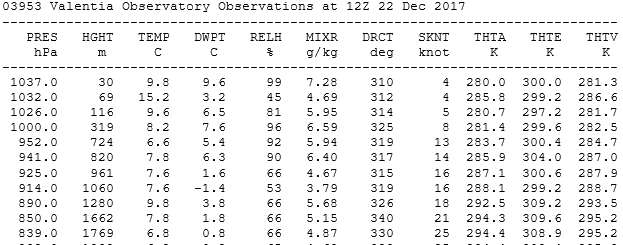
\includegraphics[width=0.4\textwidth]{Dat.PNG}
 \end{figure}
\bigskip
Como se borraron los títulos de cada columna, declaramos de nuevo los nombres de los datos. El archivo también incluía en las últimas líneas datos basura que no servían, por lo que también fueron eliminadas.  Además, como la siguiente fila eran líneas y no los datos aún, por separado hicimos que también ignorara esa línea:
\bigskip
\begin{figure}[h!]
 \centering
  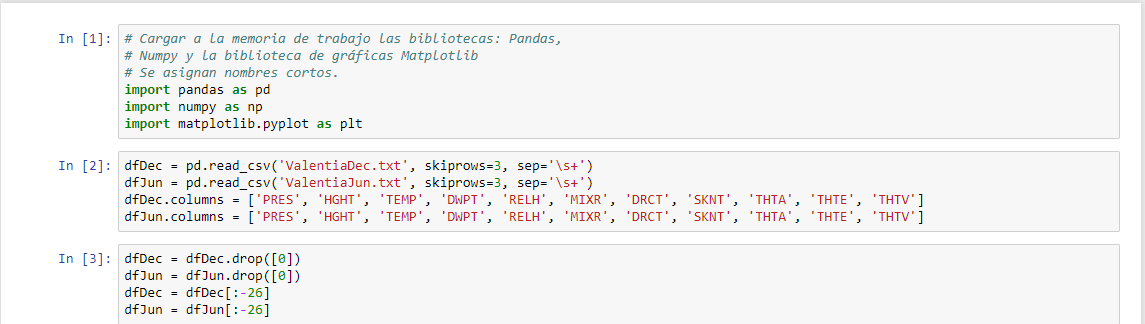
\includegraphics[width=0.6\textwidth]{LecDat1.PNG}
 \end{figure}
 \bigskip
 Con esto, los datos ya se leían correctamente, pero aquí se presentó otro problema, algunos datos no se consideraban números, por lo que se forzó a que considerara a todos como números:
 \bigskip
 \begin{figure}[h!]
 \centering
  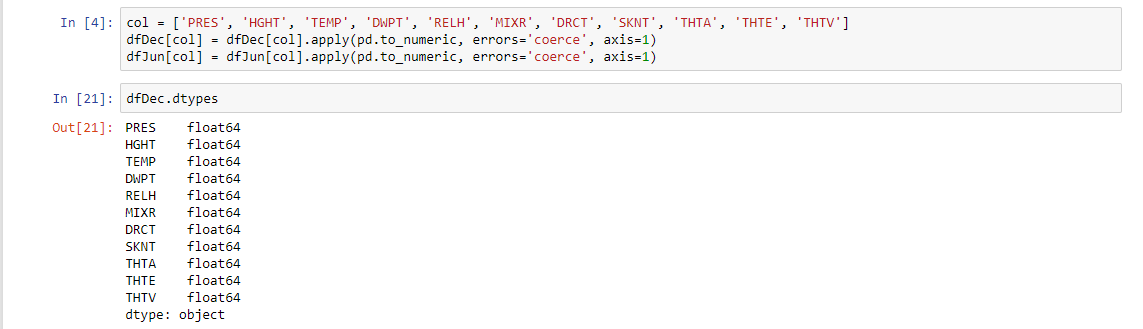
\includegraphics[width=0.6\textwidth]{LecDat2.PNG}
 \end{figure}
 \bigskip
 Se revisaron los datos una última vez, para asegurar que los datos estén de forma correcta, mostrando el principio y el final de ellos. Con esto, los datos ya estaban listos para ser usados para crear las gráficas:
\bigskip
 \begin{figure}[h!]
 \centering
  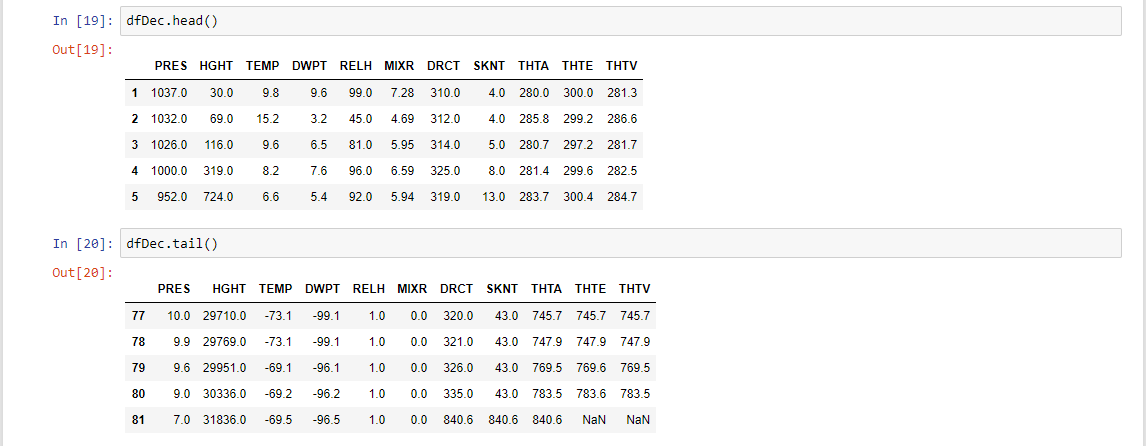
\includegraphics[width=0.6\textwidth]{LecDat3.PNG}
 \end{figure}
\bigskip

\pagebreak
\section{Resultados}
Ahora, se muestra el producto final de la actividad: las gráficas. 

\subsection{Variación de la Presión contra Altura}
\bigskip
 \begin{figure}[h!]
 \centering
  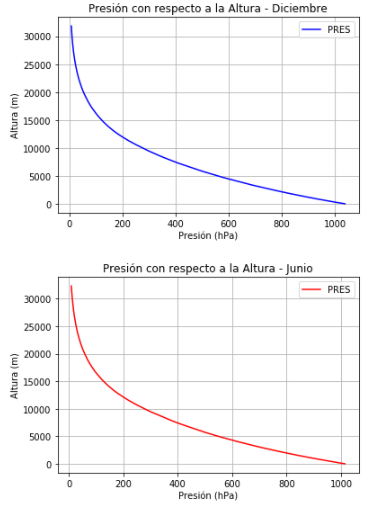
\includegraphics[width=0.8\textwidth]{Grafica1.PNG}
 \end{figure}
\bigskip

La grafica muestra como la presión va descendiendo mientras la altura aumenta.

\pagebreak
\subsection{Temperatura contra altura}
\bigskip
 \begin{figure}[h!]
 \centering
  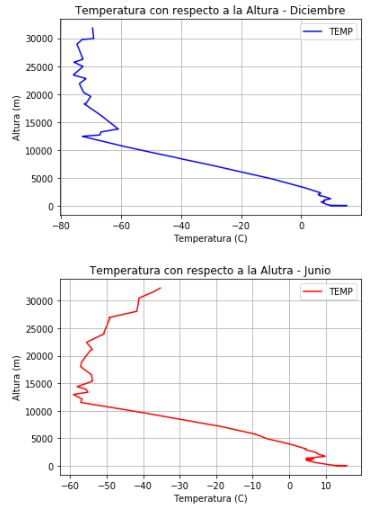
\includegraphics[width=0.8\textwidth]{Grafica2.PNG}
 \end{figure}
\bigskip

\textbf{¿Hay cambios significativos en la tropopausa entre las dos fechas?}
Sí. La tropopausa se encuentra entre los 9 y 17 km. Si buscamos en la gráfica, podemos notar que entre esos puntos donde la temperatura parece descender en un máximo, para luego volver a subir mediante adquiere altura; podemos ver que en Diciembre marca alrededor de -77$^\circ$C, aproximadamente, mientras que en Junio -60$^\circ$C aproximadamente.

\pagebreak
\subsection{Temperatura y Temperatura de Rocío contra Altura}
\bigskip
 \begin{figure}[h!]
 \centering
  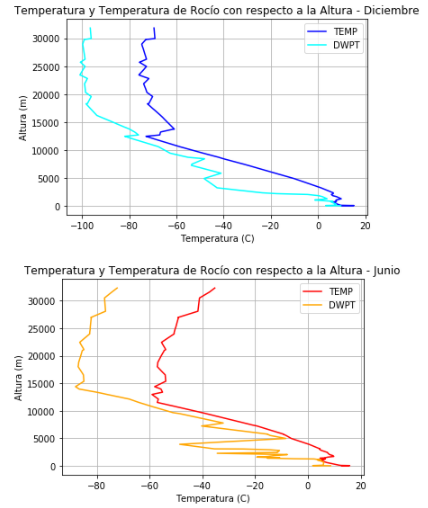
\includegraphics[width=0.8\textwidth]{Grafica3.PNG}
 \end{figure}
\bigskip

En la gráfica podemos notar como la temperatura y la temperatura del rocío van disminuyendo mientras avanza la altura. También se observa como la temperatura del rocío parece imitar e ir más bajo que la temperatura.

\pagebreak
\subsection{Rapidez de los Vientos contra Altura}
\bigskip
 \begin{figure}[h!]
 \centering
  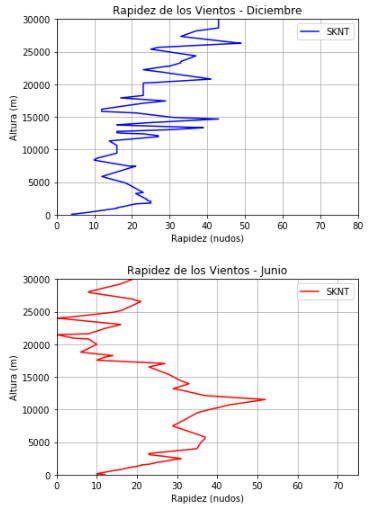
\includegraphics[width=0.8\textwidth]{Grafica4.PNG}
 \end{figure}
\bigskip
Podemos notar como en Diciembre, el viento, con algunas variaciones, parece que tiende a quedarse en un mismo rango, aumentando o descendiendo de manera leve, mientras asciende la altura. En Junio parece variar mucho, ya que primero asciende, luego desciende y luego vuelve a ascender, mientras asciende la altura.

\pagebreak
\subsection{Humedad Relativa contra Altura}

\bigskip
 \begin{figure}[h!]
 \centering
  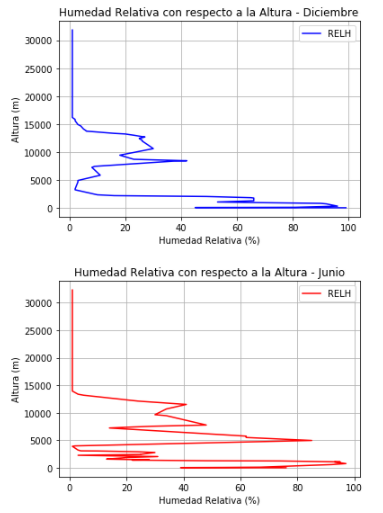
\includegraphics[width=0.8\textwidth]{Grafica5.PNG}
 \end{figure}
\bigskip

La humedad relativa en ambas gráficas parece ir variando de manera extrañas, pero se estabiliza después de los 15 km. 

\section{Conclusión}

La actividad denotó rápidamente desde un inicio lo complicado que puede llegar a ser el manejo de los datos, al momento de intentar darle una buena organización y confección, para que puedan ser detectados correctamente al momento de utilizarlos. Por otro lado, graficar fue algo mucho más sencillo. Por comparar, pulir los datos para poder utilizarlos fue un proceso muy interrumpido, ya que constantemente había que buscar en fuentes las formas para hacer ciertas modificaciones para poder estructurarlos; mientra que por el lado de la graficación, fue un proceso sistematizado, que llevaba un orden muy simple y repetitivo.   

Al final de cuentas, el objetivo general de la actividad fue completada con éxito, las graficas se lograron, junto con un análisis de los datos. Además se considera que hubo un objetivo implícito dentro de la actividad, ya mencionado en el párrafo anterior, que fue el de comprender que a veces la parte complicada es darle estructura a los datos y no tanto la parte de graficar. 


\section{Biblografía}
\begin{enumerate}
\item \begin{verbatim}
Willems, K. (2016) PAndas Tutorial: DataFrames in Python. Recuperado el
11 de Febrero del 2018 desde https://www.datacamp.com/community/
tutorials/pandas-tutorial-dataframe-python
\end{verbatim}
\item \begin{verbatim}
Albom, C. (2017) Dropping Rows And Columns In pandas Dataframe. 
Recuperado el 11 de Febrero del 2018 desde https://chrisalbon.com/python/
data_wrangling/pandas_dropping_column_and_rows/
\end{verbatim}
\item \begin{verbatim}
Wikipedia (s.f.) Atmosphere of Earth. Recuperado
el 13 de Febrero del 2018 desde https://en.wikipedia.org/
wiki/Atmosphere_of_Earth
\end{verbatim}
\item \begin{verbatim}
Wikipedia (s.f.) Atmospheric Sounding. Recuperado el 13 de Febrero
del 2018 desde https://en.wikipedia.org/wiki/Atmospheric_sounding
\end{verbatim}
\item \begin{verbatim}
Wikipedia (s.f.) Weather Ballon. Recuperado el 13 de Febrero del 2018
desde https://en.wikipedia.org/wiki/Weather_balloon
\end{verbatim}
\end{enumerate}


\section{Apéndice}
\begin{enumerate}
\item \textbf{¿Cuál es tu opinión general de esta actividad?}
Se sintió como una continuación de la actividad pasada, solo que un poco más directamente asociada a aprender a gráficar datos, más que a introducirnos a Python y sus biblotecas.
\item \textbf{¿Qué fue lo que más te agradó? ¿Lo que menos te agradó?}
Desde la práctica pasada ha sido interesante aprender más sobre Python, en especial el poder graficar tan fácil, por lo que fue lo que más me agrado. Lo que menos me agradó fue descubrir que a veces poder darle como un "retoque" y organización a los datos, para evitar cosas innecesarias, puede tomar mucho tiempo a comparación de lo fácil que es graficar. 
\item \textbf{¿Qué consideras que aprendiste en esta actividad?}
Aprendí más a fondo los comandos e instrucciones para poder organizar y retocar los datos; así como nuevas formas de darle más formato a las gráficas, como color a las líneas.  
\item \textbf{¿Qué le faltó? ¿O le sobró?}
Todo estuvo muy bien, la práctica ha sido fácil y bueno a la vez para seguir apoyando al aprendizaje de Python y a trabajar con sus herramientas.
\item \textbf{¿Que mejoras sugieres a la actividad?}
Me gustó que en las prácticas pasadas había bibliografía que mostraba herramientas y ayuda para las prácticas, por lo que me gustaría tenerlas en esta y en las prácticas que siguen. 
\end{enumerate}
\end{document}